% Created 2021-04-23 Fri 14:34
% Intended LaTeX compiler: pdflatex
\documentclass[english,zadani,odsaz]{fitthesis}
\renewcommand\title[1]{}
\projectinfo{
  project={DP},
  year={2021},
  date=\today,
  title.cs={Just-in-time překlad závisle typovaného lambda kalkulu},
  title.en={Just-in-Time Compilation\\of the Dependently-Typed Lambda Calculus},
  title.length={15.5cm},
  %sectitle.length={14.5cm}, % nastavení délky bloku s druhým titulkem pro úpravu zalomení řádku (lze definovat zde nebo níže)
  author.name={Jakub},
  author.surname={Zárybnický},
  author.title.p={Bc.},
  department={UITS},
  supervisor.name={Ondřej},
  supervisor.surname={Lengál},
  supervisor.title.p={Ing.},
  supervisor.title.a={Ph.D.},
  faculty={FIT},
  faculty.cs={Fakulta informačních technologií},
  faculty.en={Faculty of Information Technology},
  department.cs={Ústav inteligentních systémů},
  department.en={Department of Intelligent Systems},
  keywords.cs={Truffle, Virtuální stroj JVM, just-in-time překlad, tvorba překladačů, závislé typy, lambda kalkul},
  keywords.en={Truffle, Java Virtual Machine, just-in-time compilation, compiler construction, dependent types, lambda calculus},
  abstract.en={
   A number of programming languages have managed to greatly improve their
   performance by replacing their custom runtime system with general platforms
   that use just-in-time optimizing compilers like GraalVM or RPython. This
   thesis evaluates whether such a transition would also benefit
   dependently-typed programming languages or theorem provers.

   This thesis introduces the type-theoretic notion of dependent types and the
   algorithms involved in working with them, specifies a minimal
   dependently-typed language on the $\lambda\Pi\text{-calculus}$, and presents
   the implementation two interpreters for this language: a simple interpreter
   written in Kotlin, and a second interpreter, also written in Kotlin, that
   uses the Truffle language implementation framework on the GraalVM platform,
   which is a partial evaluation-based just-in-time compiler based on the Java
   Virtual Machine. The performance of these two interpreters is then compared
   on a number of normalization and elaboration tasks.

   [...specific numbers]
  }, abstract.cs={

   Řada programovacích jazyků byla schopna zvýšit svoji rychlost nahrazením
   běhových systémů, stavěných pouze pro potřeby jazyka, obecnými platformami,
   které pro optimalizaci používají just-in-time překlad, jako jsou GraalVM nebo
   RPython. Tato práce vyhodnocuje, zda je použití takovýchto platforem vhodné i
   pro jazyky se závislymi typy nebo důkazovými systémy.

   Tato práce představuje koncepty $\lambda\text{-kalkulu}$ a teorie typů
   potřebné pro úvod do závislých typů a algoritmy, které jsou potřeba pro práci
   s nimi, specifikuje malý závisle-typovaný jazyk založený na
   $\lambda\Pi\text{-kalkulu}$, a prezentuje dva interpretery tohoto jazyka:
   jednoduchý interpreter ve funkcionálním stylu psaný v jazyce Kotlin, a druhý
   interpreter, taktéž psaný v jazyce Kotlin, který používá platformu GraalVM a
   Truffle, knihovnu pro vytváření programovacích jazyků. GraalVM je platforma
   založená na virtuálním stroji Javy (JVM), která přidává just-in-time
   překladač založený na částečném vyhodnocení (\textit{partial evaluation}). Na
   závěr práce vyhodnocuje běhové charakteristiky těchto interpreterů na různých
   zátěžových testech.

   [...vyhodnocení]
  },
  extendedabstract={
  Systémy, které používají závislé typy, umožňují programátorům vytvářet
  programy, které jsou zaručeně správné vzhledem k vlastnostem, které mají
  uložené v typech. Tyto systémy je také možné použít pro logické nebo
  matematické důkazy, nebo pro dokazování správnosti celých systémů.  Poslední
  roky přinesly mnoho pokroků v teorii typů, na níž jsou tyto systémy založené,
  jako např. kvantitativní nebo homotopické typy. Vysoké nároky na důkazové schopnosti
  systémů s sebou ale prináší problémy s výkonem, konkrétně rychlostí kontroly
  typů (\textit{type-checking}, \textit{elaboration}). V této práci zhodnocuji
  vhodnost just-in-time překladu pro takové systémy, což je jeden z obecných
  přístupů pro optimalizaci rychlosti systémů.

  V první části vysvětluji principy typovaného $\lambda\text{-kalkulu}$, na němž
  jsou systémy se závislými typy založené, základy teorie typů a konkrétní
  specifikace několika rozšíření, které poté používám pro specifikaci malého
  jazyka.

  V druhé sekci pokračuji představením algoritmů, které jsou potřeba pro práci
  se závislými typy: \textit{normalization-by-evaluation} a
  \textit{bidirectional typing}. Tyto implementuji a používám pro vytvoření
  funkčního interpreteru tohoto jazyka.

  Třetí sekce představuje detaily platformy GraalVM a knihovny Truffle, které
  poté používám pro implementaci druhého interpreteru, který využívá
  just-in-time překladu.

  V závěru práce vyhodnocuji [...]

  Vyhodnocení, přínos práce
  },
  declaration={
    I hereby declare that this Master's thesis was created as an original work
    by the author under the supervision of Ing. Ondřej Lengál Ph.D.

    I have listed all the literary sources, publications, and other sources
    that were used during the preparation of this thesis.
  },
  acknowledgment={
    I would like to thank my supervisor Ing. Ondřej Lengál Ph.D. for entertaining a
    second one of my crazy thesis proposals.

    I would like to thank Edward Kmett for suggesting this idea: it has been a
    challenge.

    I would also like to thank my family and friends who supported me when I needed
    it the most throughout my studies.
  }
}

\date{\today}
\title{}
\hypersetup{
 pdfauthor={},
 pdftitle={},
 pdfkeywords={},
 pdfsubject={},
 pdfcreator={Emacs 28.0.50 (Org mode 9.3)}, 
 pdflang={English}}
\begin{document}

% * (front matter)                                              :ignoreheading:
\maketitle
\setlength{\parskip}{0pt}
{\hypersetup{hidelinks}\tableofcontents}
\iftotalfigures\listoffigures\fi
\iftotaltables\listoftables\fi
\iftotallistings\listoflistings\fi
\iftwoside\cleardoublepage\fi
\setlength{\parskip}{0.5\bigskipamount}

\chapter{Introduction}
\label{sec:org778d43f}
\section{(Old)}
\label{sec:orga7f658f}
When creating small experimental or research languages, writing a compiler may
be too much effort for the expected gain. On the other hand an interpreter is
usually not as performant as its creators may require for more computationally
intensive tasks.

There is a potential third way, proposed by Yoshihiko Futamura in the 1970s,
called the Futamura projection (or partial program evaluation), wherein an
interpreter is specialized in conjunction with the source code of a program,
yielding an executable. Some parts of the interpreter may be specialized, some
optimized, some left off entirely. Depending on the quality of the specializer,
the gains may be several orders of magnitude.

The goal of my thesis is to evaluate whether the GraalVM/Truffle platform is
suitable enough to act as a specializer for functional languages, in particular
for the dependently-typed lambda calculus.  To illustrate in Figure
\ref{fig:futamora}, the question is whether the path \textit\{Native
Image\textrightarrow Result\} is fast enough compared to the path
\textit{Executable\textrightarrow Result}.

\begin{figure}
\centering
\begin{tikzcd}
{} & Program
 \arrow[bend right]{ld}{Compiler}
 \arrow[bend right=67]{dd}{Interpreter}
 \arrow[bend left]{rd}{Partial Evaluation}
 \arrow[bend left=67]{dd}{JIT} & {} \\
Executable \arrow[bend right]{rd}{Run} & {} & Native\ Image \arrow[bend left]{ld}{Run}
 \\ {} & Result & {}
\end{tikzcd}
\caption{Methods of program execution}
\label{fig:futamora}
\end{figure}

Truffle has already been used rather successfully for the (mostly) imperative
languages Ruby, Python, R, Java, and WebAssembly, but (purely-)functional
languages differ in their evaluation model and in particular the required
allocation throughput, so it is still an open question whether GraalVM is a good
enough fit.

The desired outcome---at least, of the first part of my thesis---is a set of
implementations, and a set of benchmarks demonstrating a positive or a negative
result.  If the result is positive, there are many potential follow-up tasks:
implementing a different, more complex language, maybe a language to be
interpreted into the dependently-typed lambda calculus to attempt the approach
implemented in the \emph{Collapsing Tower of Interpreters} \cite{amin18_collapsing_towers},
or experimenting with different runtime models - all depending on the results of
this preliminary proof of concept.

In the best case, the JIT-compiled program would be as close in performance to a
program processed by a hand-crafted compiler as possible (not including JIT
warm-up), and I would spend the second half of my thesis on different topics
(like provably-correct program transformations) instead of hand-optimizing the
primitive operations - I should find out which it is going to be as soon in the
second term as possible.

As far as I am aware, there are no other native just-in-time compiled
implementations of the dependently-typed lambda calculus, with the exception of
the preliminary investigations done by the originator of this idea
\cite{kmett_2019}, although there are a few projects implementing a lambda
calculus directly to the Java Virtual Machine byte code..

\section{(New-ish)}
\label{sec:org4e351fa}
The aim of this work is to create an efficient compiler for a language with
dependent types. Compiling dependently-typed languages, compared to simply-typed
or untyped languages, comes with large performance penalties, often making large
non-trivial programs hard to write due to the compiler running out of memory or
taking minutes to compile.
\url{https://github.com/agda/agda/issues/514\#issuecomment-129023737}
\url{https://github.com/idris-lang/Idris2/issues/964}
On the other hand, programming language research projects place more and more
demands on the compiler (cubical, univalence, \ldots{} CITE)

The goal of this project is to create a compiler for a dependently-typed
language that outperforms existing compilers at, in particular, the speed of
type-checking and compilation; evaluation speed of the resulting program is not
as important for our benchmarks. Special attention will be on the asymptotics,
as the implementation platform brings rather large constant factors.

This work is a successor to the Cadenza project (cite) which implements a
simply-typed lambda calculus with extensions in the Truffle framework. While it
is unfinished and did not show promising performance compared to other
simply-typed lambda calculus implementations according to its creator Edward
Kmett, my work attempts to apply its ideas to the dependently-typed lambda
calculus, where the presence of type-level computation should lead to larger
gains.

\todo[inline]{This work builds on the pedagogic and algorithmic work on DTT by A.K.}

I have not found another attempt to apply just-in-time compilation in the
implementation of a language with dependent types and in type-level computations
in particular, despite the fact that adding just-in-time compilation to the
type-checking phase of compilation seems natural in the context of
dependently-typed languages where type-level computation is available. I assume
that it is due to the fact that the Truffle project is aimed primarily at
imperative languages and mapping functional concepts is not straightforward
(\todo{luna}) - and implementing a standalone just-in-time compiler is not
straightforward.

Improving the algorithms for type-checking is an active area of research, but
implementing them in a more dynamic manner (beyond just changing the data
structures) is not something I have found.

--- Using the technique of just-in-time compilation we can avoid the performance
problems associated with dependent type-checking by rewriting inefficient parts
of the control-flow graph during compilation.

--- The Truffle language implementation framework gives us a way of turning an
interpreter into a compiler with few changes, and allows us to rewrite the
control-flow graph and just-in-time compilation process during runtime.

--- This is a novel approach to a problem all current dependently-typed
languages face and, if successful, will bring immediate benefits to programming
language implementers.

\todo[inline]{In addition (, easy) prototyping (, stepping) block for other projects (efficient LF/Twelf (, ...))}

smalltt a step in another direction

\section{New-er}
\label{sec:org0b5024f}
\textbf{Problem statement:}
\begin{itemize}
\item Just-in-time compilation has proven itself in mainstream languages (from Java, Python, \ldots{}).
\item Virtual machines and/or optimizing compilers are expensive to maintain
\item Can we use Truffle to reuse the optimizing machinery of the Java Virtual
Machine in other languages.
\end{itemize}

\textbf{Caveat}: Originally intended just as a compiler + efficient dependent λ-calculus
runtime, but due to a badly specified assignment, I had also needed to study
type theories and in particular type elaboration, which I have also attempted to
use in this thesis.

\textbf{Why?} Dependent types give more guarantees, enable correct-by-construction code,
and a way of working that resembles a dialog with the compiler. \todo[inline]{What are notable use cases? What 's been proven in Coq?}, hot ML research area (cubical, path, \ldots{}) (look in Kovacs' materials)

\textbf{How?} Lambda calculus with types and extensions.
\begin{itemize}
\item What does it look like?
\item Show realistic λ calculus code (Church encoding + μ)
\item Adding types and their effect on computability, examples of extensions (Π, Σ,
μ), complete system ΠΣ, Type:Type
\end{itemize}

\textbf{What are we doing?} Systems like this (proof assistants) exist and are relatively
widely used. Performance is a serious concern when proving properties of larger
systems (\todo{Google Decoders}) and although a large part of it are
algorithmic problems, just-in-time compilation has not been previously
investigated as a possible part of the solution - which is a question that this
thesis attempts to evaluate.

\todo[inline]{Specifically (, Truffle) is X (, can) do Y (, Z) (claims)}

Truffle also brings Native Image and polyglot capabilities, which would be
beneficial whether the performance benefits are visible or not.

\chapter{Language specification: λΠ calculus with extensions}
\label{sec:orgadcaaa0}
\section{Introduction}
\label{sec:orgc79c4c4}
\todo[inline]{To reiterate (, the) core language of proof assistants (1 para)}

\todo[inline]{More powerful than simple type systems but potentially not decidable (1 para)}

\todo[inline]{Why not reuse Agda 's core language? Goal is minimal lang + extensions (2 paras)}

\section{λ calculus}
\label{sec:org416888b}
The untyped lambda calculus is a simple language consisting of just three kinds
of forms: variables, function application, and abstraction. [\ldots{}]

\todo[inline]{Why λ-calculus (, what) is it (2 para)}

\todo[inline]{Describe syntax (1 para)}

\begin{figure}[!htpb]
\[\begin{array}{ccll}
e & ::= & x            & \text{variable} \\
  & |   & e_1~e_2      & \text{application} \\
  & |   & \lambda x. e & \text{abstraction}
\end{array}\]
\caption{Untyped λ-calculus}
\end{figure}

\todo[inline]{Examples - Church encoding (three columns (, trivial) examples)}
\section{λ→ calculus}
\label{sec:orgb259f14}
\todo[inline]{Typed λ-calculus + syntax (3 para)}

The simply-typed λ-calculus introduces the concept of types, which have separate
syntax and semantics from the language of terms. The language of terms is
extended with a fourth kind of term, type annotation. The language of types is
the universal or base type, and an arrow from between types.

\todo[inline]{This language is not turing-complete (, must) terminate}

\begin{figure}[!htpb]
\[\begin{array}{ccll}
e & ::= & x     & \text{variable} \\
  & |   & e_1~e_2 & \text{application} \\
  & |   & λ x. e & \text{abstraction} \\
  & |   & x:τ     & \text{annotation}
\end{array}\]
\[\begin{array}{ccll}
\tau & ::= & α           & \text{base type} \\
     & |   & τ → τ' & \text{composite type}
\end{array}\]
\caption{Simply typed lambda calculus}
\end{figure}

\todo[inline]{What are derivation rules (, describe) the symbols (1 para)}

\missingfigure{Write out the simplest derivation rules (5-6 items, half a page)}

\todo[inline]{Mention explicit substitution (, that) in the above it is just a part of the metatheory (para)}

\missingfigure{Write out explicit substitution example (1 figure)}

\todo[inline]{Typing rules - same as the above (, just) describe types (1 short para)}

\todo[inline]{Close the above (, motivating) example what is it good for? (1 para + 1 figure)}
\section{Lambda cube}
\label{sec:org067b0ce}
\todo[inline]{Brief lambda cube intro show what 's out there (3 para)}

\missingfigure{Lambda cube}

\todo[inline]{Derivation rules added by the lambda cube + options (, 2) columns}

\todo[inline]{In the rest of the thesis we will work with λω (1 para)}
\section{Extensions}
\label{sec:org5129b19}
\todo[inline]{Intro - comparison table with logic/tt (, Pi/Sigma) (, forall/exists) (, ...) (3 paras)}

\subsection{Π-types}
\label{sec:org0565cec}
dependent product type, dependent function type

\todo[inline]{generalization of the function space (2 paras)}

\(Π(n:ℕ). Vec(ℝ, n)\) vs \(Π(n:ℕ). ℝ\)

\todo[inline]{grammar (, specific) example (2 figures)}

Allows inductive types, eliminators, Church

\subsection{Σ-types}
\label{sec:org0fc7a89}
dependent sum type, dependent pair type

\todo[inline]{Dependent tuple/product/sum (2 para)}

\((a, b) : Σ_{x:A}. B(x)\)

\todo[inline]{grammar (, specific) example (2 figures)}

Allows datatypes/records, Cat + Functor?

\subsection{μ-types}
\label{sec:orgaaeebf4}
\todo[inline]{Recursive type (, box/unbox) (2 paras)}

\todo[inline]{Type-level recursion (, fixpoint) (, grammar) (2 paras)}

\missingfigure{Motivating example - from PiSigma?}

\subsection{Type : Type}
\label{sec:org848ca08}
\todo[inline]{Universes (, what) is the hierarchy used for (2 para)}

\todo[inline]{Weakening (cite PiSigma) but practical simplification (2 para)}

\missingfigure{Counter-example with multiple universes}
\section{Operations}
\label{sec:org9c59fd5}
\todo[inline]{α (, β) (, η) (, ...) (3 items)}

\todo[inline]{Same for all of the calculi (right?)}

\begin{itemize}
\item Equivalences:
\begin{itemize}
\item α-equivalence = structural, allows α-renaming
\item β-equivalence = allows β-reduction (function application step) ==
α-equivalence of β-normal forms
\item η-equivalence = allows η-reduction (f ≡ λx. f x)
\end{itemize}
\end{itemize}

\todo[inline]{Equality (, equivalence) (, structural) (, nominal) (2 para)}

\todo[inline]{Normal forms - nf (, hnf) (, whnf) (3 items (, describe))}

\missingfigure{Show off a normal form derivation - which operation is used when}

\todo[inline]{Evaluation models - CBN (, CBV) (, CBPV) (3 paras (, 1) figure)}
\section{Type checking, inference, elaboration}
\label{sec:orgfe512bf}
\begin{itemize}
\item type checking ( = determining whether a program is well-typed)
\item type inference ( = the process of obtaining the type of an expression from its
parts or implicits; Hindley-Milner is well-known)
\item elaboration = convert a partially specified expression into a complete,
type-correct form (\url{http://leodemoura.github.io/files/elaboration.pdf})
\end{itemize}

\todo[inline]{Describe the nomenclature (3 para)}

\subsection{Bidirectional typing}
\label{sec:orgd0472ca}
Bidirectional typing (\url{https://www.cl.cam.ac.uk/\~nk480/bidir-survey.pdf}) = now
standard approach, combines type-checking and inference, simpler to implement
even if inference is not required

\todo[inline]{Intro (, motivation) (, list) alternatives (, pros) and cons (2 para)}

\todo[inline]{Sketch the process? Write out lambda + app rules? (half a page)}

\subsection{Conversion checking}
\label{sec:orgcf45819}
Conversion checking = type (or expression) equivalence checking, includes
evaluation (NbE = full comparison of normal forms), checking equivalence ``as
described in the previous section''

\todo[inline]{Describe motivation for NbE (, the) process (, what) is a neutral (, eval/quote) (3 paras)}

\missingfigure{neutral terms}

\subsection{Glued values}
\label{sec:orgf90bf95}

\todo[inline]{Performance optimization (, unfolding) choice}
\section{Our syntax}
\label{sec:org2d46b79}
\todo[inline]{Putting this all together (, we) get...}

\missingfigure{The entire grammar}

\todo[inline]{The complete inference and evaluation rules are in Appendix X}

This looks nice: \url{https://homepages.inf.ed.ac.uk/wadler/papers/mpc-2019/unraveling.pdf}

\todo[inline]{Extend with builtins/primitives/wired-in types (, FFI) with truffle (, hole?)}
\chapter{Language implementation: Montuno}
\label{sec:orgacc5c98}
\section{Introduction}
\label{sec:org380f2d8}
We will first create an interpreter for Montuno as specified in the assignment,
and also because evaluation and elaboration algorithms from the literature are
quite naturally translated to a functional-style program, which is not really
possible in Truffle, the target implementation.

\todo[inline]{Demonstrate the 1 to 1 equivalence of funs and algos}

Also, there are plenty of pedagogic typed λ-calculus implementations in
Haskell and other functional languages, which are often literal translations of
such algorithms.

\todo[inline]{Structure - parse (, presyntax) (, bi-di) (, syntax) (, eval) (, nametable) (, REPL/UI) (2 paras)}

\todo[inline]{Technologies (, motivate) (Gradle (, Kotlin) (, JUnit) (, JLine) (, ANTLR)) (2 paras + overview table)}

\todo[inline]{Justify Kotlin - authors don 't recommend but usable and many times shorter (citation?) (1 para)}

\section{Parser}
\label{sec:org7bcfe15}
\todo[inline]{Quick look (, not) the important part. Concerns - associativity (, position) tracking (, error) recovery (3 paras)}

ANTLR is the parser to use in JVM. Several ways to consume: listener, visitor -
I've used AST transformation which is the most compact and most familiar to
other DTLC implementations which are usually in functional languages.
(listener - enter/exit function calls, visitor is similar, toAst uses recursive
calls)

\begin{minted}[]{antlr}
FILE
    : STMT (STMTEND STMT)* ;
STMT
    : "{-#" PRAGMA "#-}"
    | ID ":" EXPR
    | ID ":" EXPR "=" EXPR
    | ID "=" EXPR
    | COMMAND EXPR
    ;
EXPR
    : "let" ID ":" EXPR "=" EXPR "in" EXPR
    | "λ" LAM_BINDER "." EXPR
    | PI_BINDER+ "→" EXPR
    | ATOM ARG*
    ;
LAM_BINDER
    : ID | "_"
    | "{" (ID | "_") "}"
    ;
PI_BINDER
    : ATOM ARG*
    | "(" ID+ ":" EXPR ")"
    | "{" ID+ ":" EXPR "}"
    ;
ARG
    : ATOM
    | "{" ID ("=" TERM)? "}"
    ;
ATOM
    : "[" ID "|" FOREIGN "|" TERM "]"
    | EXPR "×" EXPR
    | "(" EXPR ("," EXPR)+ ")"
    | "(" EXPR ")"
    | ID "." ID
    | ID
    | NAT
    | "*"
    | "_"
    ;
STMTEND : ("\n" | ";")+ ;
ID : [a-zA-Z] [a-zA-Z0-9] ;
SKIP : [ \t] | "--" [^\r\n]* | "{-" [^#] .* "-}" ;
// pragma, command discussed in text
\end{minted}

\begin{minted}[linenos,firstnumber=1]{antlr}
grammar Montuno;
@header {
package montuno;
}

file : END* decls+=top? (END+ decls+=top)* END* EOF ;
top
    : id=IDENT ':' type=term                   #Decl
    | id=binder (':' type=term)? '=' defn=term #Defn
    | cmd=COMMAND? term                        #Expr
    ;
term
    : 'let' id=binder ':' type=term '=' defn=term 'in' body=term #Let
    | LAMBDA (rands+=lamBind)* '.' body=term                     #Lam
    | (spine+=piBind)+ ARROW body=term                           #Pi
    | rator=atom (rands+=arg)* (ARROW body=term)?                #App
    ;
arg
    : '{' (IDENT '=')? term '}' #ArgImpl
    | atom                      #ArgExpl
    | '!'                       #ArgStop
    ;
piBind
    : '(' (ids+=binder)+ ':' type=term ')'    #PiExpl
    | '{' (ids+=binder)+ (':' type=term)? '}' #PiImpl
    ;
lamBind
    : binder                   #LamExpl
    | '{' binder '}'           #LamImpl
    | '{' IDENT '=' binder '}' #LamName
    ;
atom
    : '(' term ')'             #Rec
    | IDENT                    #Var
    | '_'                      #Hole
    | '*'                      #Star
    | NAT                      #Nat
    | '[' IDENT '|' FOREIGN? '|' term ']' #Foreign
    ;
binder
    : IDENT #Bind
    | '_' #Irrel
    ;

IDENT : [a-zA-Z] [a-zA-Z0-9']*;
NAT : [0-9]+;
COMMAND : '%elaborate' | '%normalize' | '%parse';

END : (SEMICOLON | NEWLINE) NEWLINE*;
fragment SEMICOLON : ';';
fragment NEWLINE : '\r'? '\n' | '\r';
SPACES : [ \t] -> skip;
LINE_COMMENT : '--' (~[\r\n])* -> skip;
BLOCK_COMMENT : '{-'~[#] .*? '-}' -> skip;
LAMBDA : '\\' | 'λ';
ARROW : '->' | '→';
FOREIGN : [^|]+;
\end{minted}

\section{Representing functions}
\label{sec:org071d325}
The main requirement for a λ calculus runtime system is fast function
evaluation, which is where we will start.

\todo[inline]{Three constructs - lam (, app) (, var) (1 para)}

A closure consists of an unapplied function, and an environment that \emph{closes over}
the free variables used in the function.

HOAS is a specific representation of closures, wherein the function is
represented as function in the host language, using the host language's support
for closing over free variables.

While representing functions using HOAS produces very readable code and in some
cases e.g. on GHC produces code an order faster than using explicit closures,
this is not possible in for us, where function calls need to be nodes in the
program graph and therefore objects, as we will see in Chapter \ref{truffle}, so
we will represent closures using explicit closures in the pure interpreter as well.

\todo[inline]{Cite Kovacs benchmarks where HOAS on GHC wins}

\todo[inline]{HOAS vs Closure code example}

\todo[inline]{Single versus multi-argument (1 para)}

\todo[inline]{Resulting data structure (TLam (, VLam) (, VCl)) (1 figure)}

\section{Representing environments and variables}
\label{sec:org3a38fad}
The way we define functions leads us to environments (Γ), which is a context
where we will look for variables.

\todo[inline]{Named versus nameless representation (2 paras (, example))}

As we saw in \todo{Where 's WHNF?}, evaluation in λ-calculus is defined
in terms of α- and β-reductions. Verifying expression equivalence also uses
variable renaming. However, traversing the entire expression in the course of
function application and applying substitution is not efficient and there are
several alternative ways.

\todo[inline]{Find de Bruijn motivating example}
\todo[inline]{Find side-by-side dB examples}

All three of them mentioned here work by replacing variable names with their
indices in a variable stack, informally \emph{counting the lambdas}.

\begin{itemize}
\item de Bruijn indices - well-known, starting from the current innermost λ
\item de Bruijn levels - less well-known, starting from the outer lambda, stable
\item locally-nameless - dB indices for bound variables,, names for free variables
\end{itemize}

Given an environment stack, indices count from the start of the stack, levels
count form the bottom. Two ways of indexing the environment, indices useful for
a stable context, levels without a stable context.

We use both, indices when quoting evaluated values.

\todo[inline]{Environments - arrays (, cons) lists (, stack) (, mutable/immutable) (2 paras)}

\todo[inline]{Snippet of code - binding a variable (, looking) up a variable (1 figure)}

\section{Evaluation algorithm}
\label{sec:org7ecab65}
\todo[inline]{Equals (W) (H) NF (, Single-variable) functions - trivial transcription (1 para)}

\todo[inline]{What are our neutrals (1 para?)}

\todo[inline]{Eval Quote (, very) briefly (2 paras)}

\todo[inline]{Extensions (Pi (, Sigma) (, Eta) (, ...)) (2 paras)}

\section{Type checking and elaboration}
\label{sec:orgaf09188}
\todo[inline]{Approach - infer (, check) + eval/quote used (, global) contexts (2 paras)}

\todo[inline]{Metavariables and holes (, sequential) processing (1 para)}

\todo[inline]{How do we do unification (2 paras + 1 figure)}

\todo[inline]{Glued values - optimistic optimization (3 paras + 1 figure)}

\section{User interface}
\label{sec:org12cb687}
REPL

\todo[inline]{This is our UI (plus batch CLI launcher) (, what) does JLine require? (2 paras)}

\todo[inline]{State keeping - load (, reload) + querying the global state (1 para)}

commands:
\begin{itemize}
\item \texttt{:l} create a NameTable
\item \texttt{:r} recreate a NameTable
\item \texttt{:t} inferVar, print unfolded
\item \texttt{:nt} inferVar, print glued
\item \texttt{:n} inferVar type, gQuote term, show
\item \texttt{:e} print elaboration output including all metas
\end{itemize}

\missingfigure{Example CLI session}

\section{Result}
\label{sec:orgcb63eb2}
\todo[inline]{Quick look at everything that this toy can do (2-3 examples?)}

Evaluation, simplification, elaboration with holes, unification using eqRefl

Error reporting

\chapter{Designing elaboration and evaluation benchmarks}
\label{sec:org5be75a2}
equivalent programs for a few dependently-typed languages

\todo[inline]{Agda (, Idris) + cooltt (, smalltt) (, redtt) (, cubicaltt) (, ...) (2 paras)}

\todo[inline]{Also mainstream functional languages - Clojure (, GHC) (, ...) (1 para)}

\todo[inline]{We 're interested in asymptotics - effects of JIT (, not) constant factors (1 para)}

\section{Tasks}
\label{sec:orga159793}
\begin{itemize}
\item evaluation, normal form, simplification
\item elaboration, filling holes
\item known problems?
\end{itemize}

\section{Specific tasks}
\label{sec:org02a58f8}
\begin{itemize}
\item Nats - large type elaboration, call-by-need test
\item Nats - type-level calculation
\item Nats - value-level calculation
\item Nats - equality/forcing
\item Functions - nested function elaboration, implicits
\item Functions - embedded STLC?
\item pairs - large type elaboration, call-by-need test
\item pairs - nested accessors
\end{itemize}

\section{Specific languages}
\label{sec:org3b1dcac}
SmallTT, Coq, Agda, GHC - for comparison

memory profile from GHC's RTS for agda/idris/smalltt (+RTS -p)
(what about coq? - \url{https://github.com/coq/coq/blob/master/dev/doc/profiling.txt})
Graal's default memory profiler

hyperfine to benchmark - measures speed
(what about \texttt{prof}?)
memory profile from stderr output

\begin{itemize}
\item from SmallTT project, from Idris project
\item memory usage (curve)
\item compilation speed (type-heavy test)
\item evaluation speed (compute-heavy test)
\end{itemize}

\section{Results: a starting point}
\label{sec:org4efd256}
\todo[inline]{Results}

\chapter{\label{orgb20d10e}Adding JIT compilation to Montuno: \(Montuno_{Truffle}\)}
\label{sec:org0f1cd89}
\section{Self-optimizing interpreters}
\label{sec:org5cfa740}
\subsection{Classical}
\label{sec:org3f32ded}

\subsection{Tracing}
\label{sec:orgde6ed6e}

\subsection{Rewriting}
\label{sec:orga14026e}
\section{GraalVM and the Truffle Framework}
\label{sec:org8db15c0}
% *** Motivation                                                :ignoreheading:

\textbf{GraalVM} is an Oracle research project that was originally created as a
replacement for the HotSpot virtual machine written in C++. \todo{Cite Oracle} It has since expanded to include other features novel to the Java world.
The project consists of several components, the main ones being:

\textbf{Graal} is an optimizing just-in-time compiler based on partial evaluation. Graal
uses the JVM Compiler Interface which allows the main JVM to offload compilation
to external Java code. It can also use C1 (the old JVM JIT) which implies tiered
compilation (\ldots{}disabled with \texttt{-XX:-TieredCompilation}). When using the GraalVM,
the only JVMCI-compatible compiler is Graal, so automatically
used. \todo{Simplify language}

\textbf{SubstrateVM} is an alternative virtual machine that uses aggressive ahead-of-time
compilation \todo{Cite SubstrateVM} of Java bytecode into a standalone
executables, a so-called /Native Image. The project aims to guarantee fast
start-up times, relatively small binary files, and low memory footprint---as
opposed to slow start-up times due to JIT compilation and large memory usage
common to JVM-based languages.

\textbf{Truffle} (and \textbf{Truffle DSL}) is a language implementation framework, a set of
libraries that expose the internals of the Graal compiler to interpreter-based
language implementations. It promises that its users only need to write an
interpreter with a few framework-specific annotations in order to automatically
gain:
\begin{itemize}
\item access to all optimizations available on the Java Virtual Machine
\item debugger support
\item multi-language (\emph{polyglot}) support between any other Java-based or
Truffle-based languages (currently JavaScript, Python, Ruby, R, C, C++, WebAssembly)
\item the ability to gradually add optimizations like program graph rewriting,
node specializations, or inline instruction caching
\end{itemize}

(\begin{center}
\includegraphics[width=.9\linewidth]{/home/inuits/Downloads/graalvm-190721074229.pdf}
\end{center})

\todo[inline]{images from https://www.slideshare.net/jexp/polyglot-applications-with-graalvm} 

GraalVM is also intended to allow creating \emph{polyglot applications} easily,
applications that have their parts written in different languages. It is
therefore easy to e.g. call R to create visualizations for the results of a
Python program, or to call any Truffle language from Java.

This seems like a good middle ground between spending large amounts of time on
an optimized compiler, and just specifying the semantics of a program in an
interpreter that, however, will likely not run quickly.

While GraalVM/Truffle is open-source and released under GPL v2, an
enterprise edition that claims large performance improvements is released
commercially.

\begin{figure}[!htb]
\centering
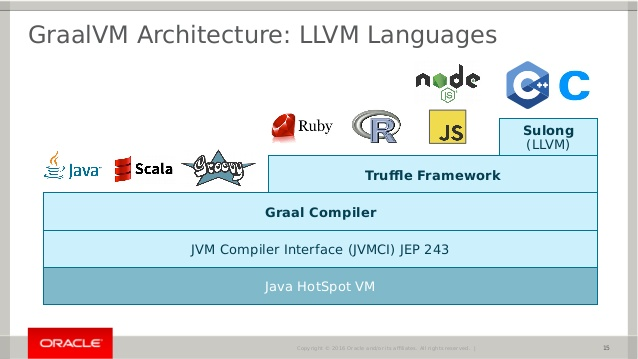
\includegraphics[width=.9\linewidth]{./img/graalvm.jpg}
\caption{GraalVM and Truffle (source: oracle.com)}
\end{figure}

\subsection{GraalVM}
\label{sec:org3ecd155}
Graal-compiled code still runs on the original HotSpot VM (written in C++)

Graal is also a graph optimizer, which takes the data-flow and instruction-flow
of the original program and is able to reorder them to improve performance. It
does what the original HotSpot VM would do, optimize JVM bytecode by reordering,
pre-compiling, or entirely rewriting instructions.

\begin{itemize}
\item Canonicization: constant folding, simplification
\item Global value numbering: prevents same code from being executed multiple times
\item Lock coarsening: simplifies \texttt{synchronized} calls
\item Register allocation: data-flow equals the registers required, optimize
\item Scheduling: instruction-flow implies instruction order
\end{itemize}

Graal by itself is just better HotSpot, but there are other technologies in the
mix. SubstrateVM is an ahead-of-time compiler for Java which takes Java bytecode
and compiles is into a single binary, including the Graal runtime, pre-compiling
application code to greatly reduce warm up times (that are otherwise shared by
all JIT compilers).

In the ideal world, what GraalVM can do with the code by itself would be enough,
if that is not sufficient then we can add specializations, caches, custom
typecasts, \ldots{} We can also hand-tune the code, adding our hand-generated
bytecode into the mix.

(Also, some fighting with Java 9 modules (closed compilation units with explicit
imports and module interfaces, needed to explicitly disable export control.))

\subsection{Truffle}
\label{sec:orgb2ea7c1}
Graal compiles ``hot code'' to machine code by partially evaluating it. Partial
evaluation is TODO (Futamora). In particular, in dynamic languages it helps to
eliminate dynamic dispatch / megamorphic call overhead.

Basic case is type specialization - when an addition node only encounters
integers, there is no need to generate machine code for floats, doubles, or
operator overloads - only verified by fast checks. When these fail, the node is
de-optimized, and eventually re-compiled again.

Inline caching for e.g. method lookups, virtual method calls are typically only
ever invoked on a single class, which can be cached, and the dispatch node can
be specialized, perhaps even inline the operation.

Specializations are general, though, and nodes can go be specialized on
arbitrary conditions, using custom assumptions and \emph{compilation final} values. In
general, node states form a directed acyclic graph - ``a node can ever become more
general''.

Using a graph visualizer, we can look at this process on a simple example
commonly used to demonstrate this part of the Truffle framework: the \texttt{+}
operation.

\todo[inline]{label}
\begin{minted}[]{kotlin}
abstract class LangNode : Node() {
    abstract fun execute(frame: VirtualFrame): Any
}
class IntLiteralNode(private val value: Long) : LangNode() {
    override fun execute(frame: VirtualFrame): Any = value
}
abstract class AddNode(
    @Child val left: LangNode,
    @Child val right: LangNode,
) : LangNode() {
    @Specialization
    fun addInt(left: Int, right: Int): Int = left + right
    @Specialization
    fun addString(left: String, right: String): String = left + right
    @Fallback
    fun typeError(left: Any?, right: Any?): Unit = throw TruffleException("type error")
}
\end{minted}

The Truffle framework is said to be a domain-specific language, which in this
case means a library, a set of annotations, and a code generator. This code
generator finds classes that inherit from the \texttt{Node} class and generates, among
others, the logic behind switching specializations.

The program graph is formed from a tree of Truffle \texttt{Nodes} from which we derive
our language-specific base class, \texttt{LangNode} in this case. We define two classes
that inherit from this class, one representing integer literals, and one for the \texttt{+}
operator.

The abstract method \texttt{execute} in \texttt{LangNode} is the evaluation of this node. It takes
a \texttt{VirtualFrame}, which represents a stack frame, and its return value is also the
return value of the node. In addition, methods starting with \texttt{execute} are special
in Truffle. Truffle will pick the most appropriate one based on return type
(with \texttt{Any} being the most general) and parameters.

In \texttt{IntLiteralNode} we directly override the method \texttt{execute}, as there is only one
possible implementation. In \texttt{AddNode}, however, we keep the class abstract and
don't implement \texttt{execute}, and instead rely on Truffle to generate the appropriate
specialization logic.

Truffle will decide between the specializations based on parameter types, and on
user-provided guards (we'll see further). Fallback specialization matches in
cases where no other one does. Names are irrelevant.

(Maybe show generated code?) Active an inactive specializations: can be multiple
active, execute method is based on state first, and only then on type checks -
smaller and possibly better optimized result. If no specialization matches, then
fall through to \texttt{executeAndSpecialize} which invalidates any currently compiled
using \texttt{CompilerDirectives.transferToInterpreterAndInvalidate} and sets state bits
for newly activated specializations.

(@Specialization(Replaces=[``'']))


How to run? Need to wrap in a \texttt{RootNode}, which represents executable things like
methods, functions and programs. Then create a \texttt{CallTarget} using
\texttt{Truffle.getRuntime().createCallTarget(root)}. Truffle uses CallTargets to record,
among others, how often a particular graph is called, and when to compile
it. Also it creates a VirtualFrame for this call target out of the provided
arguments.

IGV receives JIT compilation output - shows the Graal graphs produced during
optimization. Compilation is only triggered after a certain threshold of calls,
so we need to run a call target more than just once.

\todo[inline]{Graal-graph}


Another option: a CountNode (public int counter; execute = counter++). Green ==
state, grey is floating (not flow dependent), blue lines represent data flow
(data dependencies), red means control flow (order of operations)

Another visualization option: Seafoam

\noindent\rule{\textwidth}{0.5pt}

Intro + motivating multilanguage snippet

\todo{Self-optimizing AST interpreters (tracing (, JIT))}

features with code samples

benchmarks for other languages

JIT options - specialization, deoptimization
Use cases
Potential optimizations
Databases

\begin{minted}[]{text}
N: unbounded
P: N for exclusive, 1 for shared context policy
L: number of installed languages
I: number of installed instruments

- 1 : Host VM Processs
 - N : Engine
   - N : Context
     - L : Language Context
   - P * L : TruffleLanguage
   - I : Instrument
     - 1 : TruffleInstrument
\end{minted}

\subsection{Truffle specific features}
\label{sec:orgbc58382}
\begin{itemize}
\item RootNode - can be made into a CallTarget. is at the root of a graph, ``starting
point of a function/program/builtin'', ``callable AST''
\item OSM (Object Storage Model) - Frame (\textasciitilde{}typed HashMap)
\item VirtualFrame - virtual/optimizable stack frame, ``a function's/program's scope''
\item MaterializedFrame - VirtualFrame in a specific form, not optimizable, can be
stored in a ValueType
\end{itemize}

\section{Inspiration}
\label{sec:org19ef1ec}
\subsection{Mumbler}
\label{sec:orgadacfc9}

\subsection{Truffled PureScript}
\label{sec:org69ada9d}
Old project, but one of the only purely-functional Truffle languages.

Purescript is a derivative of Haskell, originally aimed at frontend
development. Specific to Purescript is eager evaluation order, so the Truffle
interpreter does not have to implement thunks/delayed evaluation.

Simple node system compared to other implementations:
\begin{itemize}
\item types are double and Closure (trivial wrapper around a RootCallTarget and a MaterializedFrame)
\item VarExpr searches for a variable in all nested frames by string name
\item Data objects are a HashMap
\item ClosureNode materializes the entire current frame
\item AppNode executes a closure, and calls the resulting function with a \{ frame, arg \}
\item CallRootNode copies its single argument to the frame
\item IR codegen creates RootNodes for all top-level declarations, evaluates them,
stores the result, saves them to a module Frame
\item Abstraction == single-argument closure
\end{itemize}

\subsection{FastR}
\label{sec:orgb5af711}
Replacement for GNU R, which was ``made for statistics, not performance''

Faster without Fortran than with (no native FFI boundary, allows Graal to
optimize through it)

Interop with Python, in particular - scipy + R plots

\begin{minted}[]{kotlin}
val ctx = Context.newBuilder("R").allowAllAccess(true).build();
ctx.eval("R", "sum").execute(arrayOf<Int>(1,2,3));
\end{minted}

\begin{minted}[]{r}
benchmark <- function(obj) {
    result <- 0L
    for (j in 1:100) {
       obj2 <- obj$objectFunction(obj)
       obj$intField <- as.integer(obj2$doubleField)
       for (i in 1:250) { result <- obj$intFunction(i, obj$intField) }
    }
    result
}
benchmark(.jnew("RJavaBench"))
\end{minted}

Special features:
\begin{itemize}
\item Promises (call-by-need + eager promises)
\end{itemize}

\subsection{Cadenza}
\label{sec:org75211c7}

\begin{itemize}
\item FrameBuilder - specialized MaterializedFrame
\item Closure - rather convoluted-looking code
\end{itemize}

Generating function application looks like:
\begin{itemize}
\item TLam - creates Root, ClosureBody, captures to arr, arg/envPreamble
\item Lam - creates Closure, BuilderFrame from all captures in frame
\item Closure - is a ValueType, contains ClosureRootNode
\item ClosureRootNode - creates a new VirtualFrame with subset of frame.arguments
\end{itemize}

\subsection{Enso}
\label{sec:org7c71c80}
A very late addition to this list, this is a project that originally rejected
Truffle (and dependent types in general, if I recall correctly) and used Haskell
instead. However, the project Luna was renamed to Enso, and rebuilt from scratch
using Truffle and Scala not long before my thesis deadline. 

\section{Truffle Interpreter}
\label{sec:org5552eae}
% *** Intro                                                     :ignoreheading:
Truffle is not primarily aimed at statically-typed languages or functional
languages. Its most easily accessible benefits lie in speculative optimization
of dynamically typed code and inline caches, where generic object-oriented code
can be specialized to a specific value type. Statically-typed languages have a
lot more information regarding the values that will flow through a function, and
e.g. GHC has a specific \emph{specialization} compiler pass.

However, there is a lot of overlap between the static optimizations done by
e.g. GHC and runtime optimizations done by Graal. An example would be
unfolding/inlining, where the compiler needs to make a single decision of
whether to replace a call to a function with its definition -- a decision that
depends on the size of the definition, whether they are in the same module, and
other heuristics (\todo[inline]{https://www.microsoft.com/en-us/research/wp-content/uploads/2002/07/inline.pdf}). A Truffle interpreter would be able to postpone the decision
until execution time, when the definition could be inlined if the call happened
enough times.

Its execution model is a tree of nodes where each node has a single operation
\texttt{execute} with multiple specializations. The elaboration/evaluation algorithm from
the previous chapter, however, has several interleaved algorithms (infer, check,
evaluate, quote) that we first need to graft on to the Truffle execution model.

There are also several features that we require that are not a natural fit for
it, but where we can find inspiration in other Truffle languages. In particular,
lazy evaluation (FastR promises), partial function application (Enso), ???

We also have several options with regard to the depth of embedding: The most
natural fit for Truffle is term evaluation, where a term could be represented as
a value-level Term, and a CallTarget that produces its value with regard to the
current environment. We can also embed the bidirectional elaboration algorithm
itself, as a mixture of infer/check nodes.

There are several concerns here:
\begin{itemize}
\item algorithmic improvement is asymptotic -- the better algorithm, the better we
can optimize it
\item Truffle's optimization is especially applicable to ``hot code'', code that is
ran many times, e.g. a loop
\item We need to freely switch between Term and Value representations using
eval/quote
\end{itemize}

The representation is also quite different from the functional interpreter where
we've used functions and data classes, as in Truffle, all values and operations
need to be classes.

\noindent\rule{\textwidth}{0.5pt}

Kotlin seems not to be recommended by Truffle authors
(\url{https://github.com/oracle/graal/issues/1228}), but there are several languages
implemented in Kotlin, which suggests there are no severe problems.

\noindent\rule{\textwidth}{0.5pt}

evaluation phases - translate to Code, run typecheck, run eval vs glued, ???

slightly impractical compared to the functional version, subclasses with methods
instead of plain functions -> required for truffle annotations

truffle specifics

inline cache, tail call, trampoline (continuations)

!! show their effect on program graphs

native image

\subsection{Frames}
\label{sec:orgff1edf6}
FrameDescriptor - shape of a frame
FrameSlot
FrameSlotKind

VirtualFrame - can be optimized, reordered

MaterializedFrame - an explicit Java Object on the heap, created from a
VirtualFrame by calling \texttt{frame.materialize()}

\subsection{Calling convention}
\label{sec:orge8458d6}

\begin{enumerate}
\item Evaluation order
\label{sec:orgceb7304}
Call-by-need - a computation happens in the place where a value is used, and not
created (\texttt{const 5 expensiveFunc} doesn't \emph{force} the expensive computation)

Call-by-value - a computation happens immediately, whenever a value is created
(in the previous example both 5 and \texttt{expensiveFunc} would first be evaluated
before calling \texttt{const})

Call-by-push-value - formalism subsuming both (by means of a translation
strategy), defining a single evaluation order in terms of operations with a
stack - two additional operators, \textbf{distinguishes values and computations}
(including dependent types, in the original 1999 paper), operator \(U\) (delay)
creating a \emph{thunk}, and operator \(F\) (force) that forces the computation of a
delayed value/thunk.

\begin{figure}
\[\begin{array}{ccll}
A & ::= & U B | Σ(i∈I)A_i | 1 | A × A \\
B & ::= & F A | Π(i∈I)B_i | A → B
\end{array}\]
\caption{Call-by-push-value values and computations}
\end{figure}

\begin{itemize}
\item value of type \(UB\) is a thunk producing a value of type \(B\)
\item Σ is a pair (tag, Value)
\item type A × A' is a value of type (V, V')
\item type 1 is a 0-tuple
\item computation of type \(FA\) produces a value of type A
\item computation Π pops a tag \(i\) from operand stack, then is a computation of type \(B\)
\item computation A → B pops a value of type A, then behaves as type B
\end{itemize}
\todo[inline]{https://www.cs.bham.ac.uk/~pbl/papers/tlca99.pdf}

\item Calling convention
\label{sec:org1fb300b}
push-enter - arguments are pushed onto the stack, the function then takes as
many as it requires

eval-apply - the caller sees the arity of the function and then decides whether
it is over-applied (evaluates the function and creates a continuation), appllied
exactly (EVAL), or under-applied (creates a PAP, a closure-like value)

-- exactly describe the rules from eval-apply paper KNOWNCALL, EXACT, CALLK, PAP
-- known application ( = known arity), unknown function

\item Implementation
\label{sec:org35a073e}

Passing arguments - the technical problem of copying arguments to a new stack
frame in the course of calling a function.

[[Despite almost entirely re-using the Enso implementation of function calls, with
the addition of implicit type parameters and without the feature of default
argument values,

I will nonetheless keep my previous analysis of calling conventions in
functional Truffle languages here, as it was an important part of designing an
Truffle interpreter and I spent not-insignificant amounts of time on it.

I have discovered Enso only a short while before finishing my thesis, and had to
incorporate the technologically-superior solution

Several parts of creating an AST for function calls:
\begin{itemize}
\item determining the position of arguments on the original stack - or evaluating
and possibly forcing the arguments
\item determining the argument's position on the stack frame of the function
\item using this position in the process of inferring the new function call
\item dispatch, invoke, call nodes???
\end{itemize}

\todo[inline]{First (, describe) strictness analysis + CBN/V/PV (, only) then function calls}
\end{enumerate}

\chapter{Making \(Montuno_{Truffle}\) fast}
\label{sec:org402d286}

\section{Profiling}
\label{sec:orgfdb1f9d}
\subsection{Ideal Graph VIsualizer}
\label{sec:org5c89a95}
A graphical program that serves to visualize the process of Truffle graph
optimization. When configured correctly, the IGV will receive the results of all
partial evaluations.

\subsection{CPU Sampler}
\label{sec:orgd40da8c}
Running the language launcher with the options \texttt{-{}-cpusampler
-{}-cpusampler.Delay=MILLISECONDS} will start the CPU sampler. This tool serves to
profile the guest language (as opposed to the regular JDK Async Profiler which
will profile the entire process.

\texttt{-{}-cpusampler.Delay} helps to not include warm-up time in the results.

Using additional options (\texttt{-{}-cpusampler -{}-cpusampler.SampleInternal
-{}-cpusampler.Mode=roots -{}-cpusampler.Output=json}) and postprocessing the
generated JSON with an additional script we
can create a so-called flamegraph with the results of the sampling.

\section{Specializations}
\label{sec:org59f6718}
\subsection{Debugging specializations}
\label{sec:orgf225aa5}
\textbf{Specialization histogram:} If compiled with
\texttt{-Atruffle.dsl.GenerateSpecializationStatistics=true} and executed with
\texttt{-{}-engine.SpecializationHistogram}, Truffle DSL will compile the nodes in a
special way and show a table of the specializations performed during the execution of a
program.

Example shown at
\url{https://github.com/oracle/graal/blob/master/truffle/docs/SpecializationHistogram.md},
maybe include the table?

\textbf{Slow path only:} If compiled with \texttt{-Atruffle.dsl.GenerateSlowPathOnly=true},
Truffle will only execute the last, most generic specialization, and will
ignore all fast path specializations.

\chapter{Evaluation: Is \(Montuno_{Truffle}\) fast enough?}
\label{sec:orgc3a5ddb}
\chapter{Conclusion}
\label{sec:orgd3fcece}
next work: LF, techniques, extensions, real language

% * (bibliography, start of appendix)                           :ignoreheading:

\makeatletter
\def\@openbib@code{\addcontentsline{toc}{chapter}{Bibliography}}
\makeatother
\begin{flushleft}

\bibliographystyle{bibstyle}
\bibliography{bibliography}

\end{flushleft}
\iftwoside\cleardoublepage\fi
\appendix
\appendixpage
\iftwoside\cleardoublepage\fi
\startcontents[chapters]
% \setlength{\parskip}{0pt}
% \printcontents[chapters]{l}{0}{\setcounter{tocdepth}{2}}
% \setlength{\parskip}{0.5\bigskipamount}
\iftwoside\cleardoublepage\fi

\chapter{Contents of the attached data storage}
\label{sec:orgcf644f0}
\ldots{}
\end{document}